\subsubsection{Messen der Sauerstoffs{\"a}ttigung (SpO2)} \label{grund-spo2-subsubsec}


Das Messen der Sauerstoffsättigung wird als Pulsoximetrie bezeichnet und ist ein nichtinvasives Verfahren zur Ermittlung der arteriellen Sauerstoffsättigung. Zunächst muss man zwischen oxygeniertem Hämoglobin (HbO2) also ein mit Sauerstoff beladenes Hämoglobin, und desoxygenierten Hämoglobin (Hb) unterscheiden, also Hämoglobin dessen Transportplätze für =2 noch verfügbar sind. Das Messprinzip der Pulsoximetrie besteht im wesentlichen auf dem unterschiedlichen Absorptionsverlauf des beladenen und unbeladenen Hämoglobins, beim einbringen von optischer Strahlung. Dieser Verlauf ist in der Abbildung 1.3 dargestellt.

%\begin{figure}[H] \centering
%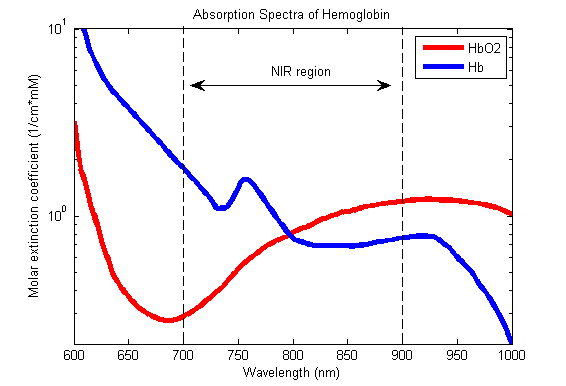
\includegraphics[width=12cm]{Images/elise_abs-Sauerstoff.png} 
%\vspace{-0.3cm} 
%\caption{Grobe {\"Abb. 1.3 Absorptionsverlauf HbO2 und Hb im Wellenlängen Bereich von 700 nm bis 900 nm.\}
%\label{fig-elise} 
%\end{figure}

Als Lichtquelle für die Messung dient eine rote und eine infrarote Leuchtdiode, als Empfänger
eine Fotodiode. Wird Sauerstoff abgegeben, d.h. nimmt die Sauerstoffsättigung im Blut ab
und verliert es seine rötliche Farbe, wird die Absorption des roten Lichts schwächer und die
des infraroten Lichts stärker. Verändert sich der arterielle Blutfluss durch das herzsynchrone Pulsieren, so wirkt dieser zusätzlich auf die Lichtabsorption ein. Die Pulswelle gibt also Veränderungen des Blutvolumens und der Bewegung der Blutgefäßwände wieder, nicht aber Veränderungen des Blutdrucks.  Da nur die Veränderung der Lichtabsorbtion ausgewertet wird, haben pulsierende absorbierende Stoffe wie Gewebe, Knochen und venöses Blut keine Auswirkung auf die Messung. Übliche Referenzwerte der Sauerstoffsättigung liegen zwischen 93 und 98 Prozent. Bei sportlicher Aktivität kann die Sauerstoffsättigung auf den maximalen Wert von 100 Prozent ansteigen. Die Messung der Sauerstoffsättigung kann aber auch verfälscht werden. Dies kann etwa durch lackierte oder künstliche Fingernägel entstehen, oder aber für uns auch relevant, durch mechanische Stöße.  
